\documentclass[a4paper]{article}

%% Language and font encodings
\usepackage[english]{babel}
\usepackage[utf8x]{inputenc}
\usepackage[T1]{fontenc}
\usepackage{minted}
\usepackage[makeroom]{cancel}
\usepackage{amsbsy}
\usepackage{physics}
\usepackage{booktabs}
\usepackage{graphicx}
\usepackage[table]{xcolor} 
\usepackage{wrapfig}

%% Sets page size and margins
\usepackage[a4paper,top=2cm,bottom=2cm,left=1cm,right=1cm,marginparwidth=1.75cm]{geometry}
\def\rcurs{{\mbox{$\resizebox{.16in}{.08in}{\includegraphics{ScriptR}}$}}}
\def\brcurs{{\mbox{$\resizebox{.16in}{.08in}{\includegraphics{BoldR}}$}}}
\def\hrcurs{{\mbox{$\hat \brcurs$}}}

%% Useful packages
\usepackage{amsmath}
\usepackage{graphicx}
\usepackage[colorinlistoftodos]{todonotes}
\usepackage[colorlinks=true, allcolors=blue]{hyperref}

\title{Deep Learning}
\author{Simple Machine Learning -> CNNs }
\begin{document}
\rowcolors{2}{gray!25}{white}
\maketitle
\section{General Machine Learning}
Machine Learning algorithms differs from "normal" algorithms because they are able to modify themselves to better solve a problem. There are many kinds of machine learning algorithms, with different strengths and weaknesses, but broadly categorized into two main groups: supervises, and unsupervised learning.

In supervised learning one provides the algorithm a training and a test data set. The training data set has some input data and associated classifications for that data, the algorithm will attempt to classify the data, then look look at the associated classifications, and then adjust itself to better match the classifications given. At the point where the algorithm can no longer make significant progress towards a more accurate classification (sometimes defined as when the true classification is within a certain amount of decimal precision, or when x number of iterations have been completed) the test data set is run through the algorithm to produce a validation score (how accurate was the model). The test data set is of identical form to the training data set, but made up of different data so as to more easily catch a model which has been over-fit to the training data. Supervised Learning therefore requires an intimate knowledge of the data one is working with, and large amounts of that data to train the model.

Unlike supervised learning, unsupervised learning does not require any hard classifications of data before hand. Unsupervised leaning attempts to locate patterns in data without knowing anything about the classification of that data. Note that unsupervised learning often requires the user to tell it how many grouping to look for. We will not focus on unsupervised learning as it is unsuitable for the goals of classifying stellar variations.

Table \ref{MLSum} summarizes different type of machine learning, however from here forward we will solely focus on Artificial Neural Networks -- the structures with form the basis for deep learning

\begin{table}
\centering
	\begin{tabular}{|p{3cm}|p{1cm}|p{5cm}|p{4cm}|p{4cm}|}
    \hline
    \textbf{Name} & \textbf{Type} & \textbf{Description} & \textbf{Error Method} & \textbf{Algorithms} \\
    \hline
    \hline
    Regression & U & Iteratively defining 1-D relationships between data and using the errors in the predicted relationship to improve the model & Standard Deviation and other standard statistical methods  & Linear Regression, Logistic Regression, Ordinary Least squares regression, stepwise regression, and others. \\
    Instance-Based & U & Build a set of 2-D relationships and attempt to minimize some goodness of fit metric (essentially 2-D state based regression) & Minimize differences between standard statistical methods (i.e. minimize the difference means of all groups for) & k-Nearest Neighbors, Locally Weighted Learning, etc.. \\
    Regularization & U & Essentially regression but a weight is added in to favor simpler models more than complex models, this helps generalize better & Same as regression but also taking complexity as a factor to be minimized & Ridge Regression, Elastic Net, and Least-Angle Regression \\
    Decision Tree & S & Build a model on a cascading set of decisions each containing a weight, which are updated at the end of each training to match the trees results more closely with the true results. & Back propagation (I believe I don't know for sure on this one) & Classification and Regression Tree, Decision Stump, Conditional Decision Tree, and M5 \\
    Clustering & U & Specifically attempts to look for groups in data by minimizing a goodness of separation metric & Goodness of separation metric, for example cluster points in two groups defined by control points, find the mean of those groups, move the control points slightly closer to the mean point then recalculate and repeat & k-Means, k-Medians, Expectational Maximization (EM) \\
    Association Rule Learning & S & Find and tweak rules that describe how one set of data transforms into another and then attempt to minimize the errors. & Back propagation (I believe I don't know for sure on this one) & Apriori Algorithm and Eclat Algorithm \\
    Artificial Neural Network (ANN) & S & Learning based on comparing all data and many perturbations of all data to each other, then back-propagating errors to modify weights to more accurately describe the data & Back-propagation or stochastic gradient decent. (to be discussed in more detail latter) & Perceptron, Hopfield Network and Deep Neural Networks (multi-layer Perceptrons), a subclass of which are Constitutional Neural networks, and Recursive neural networks. \\
    \hline
    \end{tabular}
    \caption{Summary of a few different types of machine learning. There are many more algorithms than listed here but these are some of the major ones. Nose U - Unsupervised, S - Supervised. Information from http://machinelearningmastery.com/a-tour-of-machine-learning-algorithms/}
    \label{MLSum}
\end{table}

\section{Artificial Neural Networks}
The idea of artificial neural networks (ANN) started with the Frank Rosenblatt's Perceptron in 1957\cite{Ros57}. The essential idea is that by multiplying some data by some weight one could then use stochastic gradient decent to modify that weight until it was better able to match the true result. For a number of mathy reasons that aren't particularly important it turns out that a perception is not super feasible so the idea was more or less abandoned for a while. However over the last 20-30 years algorithms have been developed which connect layers of individual perceptrons into what is called a fully-connected multi-layer perceptron, or more colloquially a deep neural network (DNN). DNNs are therefore a subclass of ANNs, however they are currently the only subclass getting much attention, and what we are using in our research so we will again adjust are focus inwards at solely DNNs.
\section{Deep Neural Networks -- pre nitty-grity}
\subsection{Cool things people are doing}
Deep Neural Networks are very common in todays world. Facebook and Google use them to identify faces in photos, Google and amazon to understand natural speech, and Microsoft is working to develop more realistic chat-bots with DNNs. Stock market trading has seen a large influx of DNNs, as has futures trading. Most applications of DNNs are currently in industrial or commercial settings. 
\subsection{What were doing}
A quick run down of what we will be doing, we hope to use DNNs to classify stars using time-series photometry as pulsators, eclipsing binaries, or plain old boring fusing balls of hydrogen which drive the universe (no stars are boring, stars are awesome). We also hope to move beyond pure classification and create a network that can predict parameters for these systems such as pulsation period, amplitude, orbital radii for eclipsing binaries, and so on. This is a very new field in astronomy with only a few papers out about it, and deep learning has never been applied to time-series photometry before.
\subsection{How Deep Learning works using words}
The structure of a small DNN can be seen in Figure \ref{DNN}. Data is passed into an input layer and then passed onto a number
\begin{wrapfigure}{r}{0.5\textwidth}
	\begin{center}
    	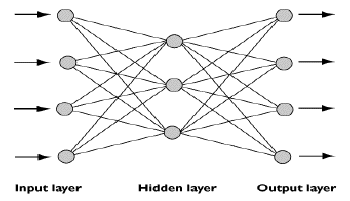
\includegraphics[width=0.48\textwidth]{DNN}
    \end{center}
    \caption{A fully-connected multi-layer perceptron (DNN)}
    \label{DNN}
\end{wrapfigure}
of hidden layers (in Figure \ref{DNN} only one hidden layer). That passing (the arrows in Figure \ref{DNN}) can be thought of as multiplications by a weight, and where arrows meet at a node the values are all summed together. That process is then repeated for each consecutive layer. eventually the hidden layers will connect to one last layer called the output layer which is where the data will be classified. So for example let us use the iris data set, this has four dimensions - pedal length (PL), pedal width (PW), sepal length (SL), and sepal width (SW) with the the goal of classifying three types iris species by these dimensions. In this case we would have four input neurons, and three output neurons. You may ask how many layers of hidden neurons and how many hidden neurons in each layer, that turns out to be a very difficult question, and one which, from my reading, appears to have no universally or even widely accepted answer. The number and depth of the hidden layers are what are called hyper-parameters, and are generally tunned manually until the user is satisfied with the outcome, but with little more guidance than that. The only real way to get any sense of a useful depth is to know that hidden neurons act as "feature detectors". For example in facial recognition a set of neurons (not necessarily on the same layer) may identify an object consistent with its idea of a nose, and another may do the same for a mouth, and eyes, and so on, until a final set compares all of those, says, "hey look all the parts of a face therefore probably a face". This is helpful as it gives the general guidance that more complex systems should probably be larger and deeper. So that is how a trained network classifies, but how is the network trained? The same process of moving multiplying, summing, and moving forward is done (this is called forward-propagation) and then the values at the output are compared to the true values, then a process known as back-propagation is preformed to adjust the weights (and bias terms witch allow for DC offsets to be introduced -- but for sake of simplicity we will only focus on the weights) in each layer based on the errors in the previous layers. Latter on we will go into more detail about that math, but know that this process essentially follow the gradient of the change in error to approach the smallest error the fastest (Note that weights are sill adjusted minuscule amounts so as to limit the possibility of over-fitting). This process is repeated a huge number of times (on the order of millions-billions) and is therefore the expensive part of DNNs (specifically back-propagation is more expensive than forward-propagation). Once the weights are dialed in however a well trained network can usually classify data significantly faster and more accurately and on a much wider (more generalized) set of data than other methods such as regression or k-means clustering.
\section{Deep Neural Networks -- The Nitty Gritty}
\subsection{Forward Propagation}
Forward propagation is the easy step, remember that in forward propagation we multiply the values at a node by weights, then sum all those at the next nodes (that was a terrible explanation but hopefully I can explain it better in person). We could do this with a series of nested loops pretty simply, however using matrix algebra allows this process to both be sped up (if we are using a language like Python MATLAB, or Lisp where native loops are slow) and made more readable. So how do we do this. Think of each layer as a matrix multiplication between some weight (W) matrix of dimension (size of layer x inputs to layer -- so for example the size of the weight matrix for the hidden layer in Figure \ref{DNN} would be 3x4) and the vector of inputs to that layer ($\vb{z}$) (note that there is also often a bias term introduced ($\vb{b}$)). So the form for each layer of forward-propagation is 
\begin{align}
	W_{i}\vb{z_{i-1}}+\vb{b_{i}} = \vb{s_{i}}
\end{align}
We run $\vb{s_{i}}$ through whats called an "activation function", these normalize the value to some range to keep weights from blowing values up, common activation function are the logistic function, hyperbolic tangent, and the Ramp Function. (I'll use the logistic function in the rest of this handout). so to get $\vb{z_{i}}$ we run $\vb{s_{i}}$ through the activation function (called activating the input) so for example if using the logistic function: 
\begin{align}
	\vb{z_{i}} = \frac{1}{1+e^{-\vb{s_{i}}}}
\end{align}
these steps are run for all the layers until the output layer. If not using an activation function with the range (0, 1) it is common to run $\vb{z_{n}}$ through a logistic function to place it in probability space. The final output is called $\vu{y} = \vb{z_{n}}$ in probability space. Thats how forward propagation works, we will not go onto to the much more complex and also interesting backwards propagation.
\subsection{Backwards Propagation}
Backwards Propagation is seemingly more complex that forward propagation, however it is important to remember that all that is happening is that the computer is following the path of fastest decrease in the absolute error between the true
\begin{wrapfigure}{r}{0.5\textwidth}
	\begin{center}
    	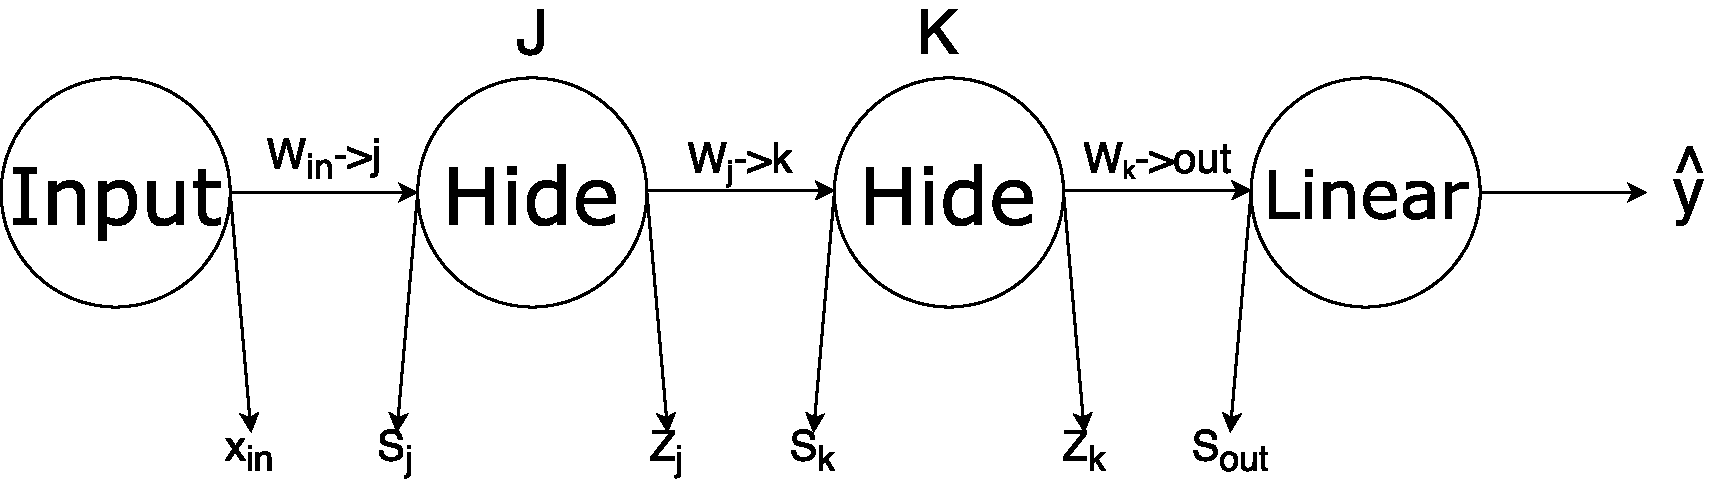
\includegraphics[width=0.48\textwidth]{jknetwork}
    \end{center}
    \caption{A DNN with input x and output $\vu{y}$}
    \label{BProp}
\end{wrapfigure}
solution and the solution that the network found. To understand the math behind this consider the network pictured in Figure \ref{BProp} made up of an input layer, two hidden layer and an output layer. We will backpropagate error through this network. First we should find the absolute error of the network $E=\frac{1}{2}(\vu{y}-\vb{y})^{2}$ where $\vb{y}$ is the true solution. Now we will define a useful metric called the error signal for the ith layer of the network $\delta_{i}=\frac{\partial E}{\partial s_{i}}$ We can rewrite this as $\delta_{i}=\frac{\partial}{\partial s_{i}}\frac{1}{2}(\vu{y}-\vb{y})^{2}$, then by the chain rule $\delta_{i}=(\vu{y}-\vb{y})\frac{\partial \vu{y}}{\partial s_{i}}$. Now we need to fork the rode, as what we do next is dependent on whether the ith layer leads to an output layer or leads to a hidden layer. Starting with if the ith layer leads to an output layer, then given some activation function $f(x)$ such that $\vu{y}=f(s_{i})$ then we can write the error signal as $\delta_{i}=(\vu{y}-\vb{y})f'(s_{i})$, we will call this $\delta_{0}$ as it is the first error signal to be calculated. Now if the ith layer does not lead to an output but to some number of hidden layers q in the output range of i ($q\in z_{i}$), then we can expand $\frac{\partial \vu{y}}{\partial s_{i}}$ via the chain rule
\begin{align*}
	\frac{\partial \vu{y}}{\partial s_{i}} &= \frac{\partial \vu{y}}{\partial z_{i}}\frac{\partial z_{i}}{\partial s_{i}}
\end{align*}
however we can see that $\frac{\partial z_{i}}{\partial s_{i}} = f'(s_{i})$ so
\begin{align*}
	\frac{\partial \vu{y}}{\partial s_{i}} &= \frac{\partial \vu{y}}{\partial z_{i}}f'(s_{i})
\end{align*}
Using the chain rule again
\begin{align*}
	\frac{\partial \vu{y}}{\partial s_{i}} &= f'(s_{i})\sum_{q\in z_{i}}\frac{\partial \vu{y}}{\partial s_{q}}\frac{\partial s_{q}}{\partial z_{i}}
\end{align*}
Note that $\frac{\partial s_{q}}{\partial z_{i}} = w_{i\rightarrow p}$ so
\begin{align*}
	\frac{\partial \vu{y}}{\partial s_{i}} &= f'(s_{i})\sum_{q\in z_{i}}\frac{\partial \vu{y}}{\partial s_{q}}w_{i\rightarrow p}
\end{align*}
substituting this into the Error signal equation from so many lines ago
\begin{align*}
	\delta_{i} = (\vu{y}-\vb{y})f'(s_{i})\sum_{q\in z_{i}}\frac{\partial \vu{y}}{\partial s_{q}}w_{i\rightarrow p}
\end{align*}
however remember that we defined error signal to be $\delta_{q} = (\vu{y}-\vb{y})\frac{\partial \vu{y}}{\partial s_{q}}$ therefore we can bring $(\vu{y}-\vb{y})$ into the summation, to finally arrive at
\begin{align}
	\delta_{i}=f'(s_{i})\sum_{q\in z_{i}}\delta_{p}w_{i\rightarrow p}
\end{align}
we can use this and $\delta_{0}$ to recursively propagate the error signal to each layer of the network. But sheet of paper you may ask "How does one use the error signal to adjust the weight matrix to each layer". I won't bother going through this derivation, the change in weights for some learning rate $\eta$, the mini-batch size N, and n number of runs will be 
\begin{align}
	\Delta w_{i\rightarrow p} = -\frac{\eta}{N}\sum_{n}\delta_{i}z_{i}
\end{align}
\section{Implementation}
One could write a network from first principals at this point, however one would be stupid to do so if one did so for any reason other than the purely pedagogical. Neural networks are not monumentally complex to program but are monumentally complex to program well. Aside from obvious pitfalls such as user introduced errors, a neural network built solely on the algorithm I have described here in python would be very slow, however there is a simple and elegant solution. Modules such as Google's Tensor Flow and Theano exist and do all of the heavy lifting when it comes to constructing, training, storing, and optimizing these networks. Modules such as Keras wrap these up in a nice pythonic blanket and make them stupid simple to use -- a network from first principals is on the oder of 100s of lines where with Keras 5 lines can construct a network. So how do we use this? I am going to leave you to install the necessary dependencies, however I will provide some tips as they can be a pain to get working.
\subsection{Basic Installation guide}
If you are on windows I recommended you install the Linux subsystem for windows, a true UNIX environment will make your life much easier.  Install anaconda, if its not installed install it and come back. I recommend you spin up a conda virtual environment
\begin{minted}{bash}
$ conda create --name ML python=3 anaconda
\end{minted}
say yes to the prompts and once that is completed
\begin{minted}{bash}
$ source activate ML
\end{minted}
then type
\begin{minted}{bash}
$ pip install tensorflow
\end{minted}
depending on your computer you may have to elevate that command. Finally type
\begin{minted}{bash}
$ pip install keras 
\end{minted}
now whenever you are in the ML virtual environment you will be able to use keras with tensorflow. When you are not in the ML environment you will not. You can launch Jupyter Notebooks from within the environment, and do anything else you would normally do. When you want to close it just type 
\begin{minted}{bash}
$ source deactivate ML
\end{minted}
\subsection{Your first network with Keras}
Our goal will be to classify the iris data-set. This is a data set with 150 rows, each containing data on Sepal Length, Sepal Width, Pedal Length, and Pedal Width and Species. Overall there are three species the goal is to classify them using the four dimensions of data. We will therefore have a four input and three output network. Each output represents a probability that that that data falls into that species. Since the species are given as string but we need a vector representing true probability for each we will use "one-hot-encoding" this essentially takes a set of strings containing n possibilities and makes a vector of length n with a one at the true value zeros elsewhere. Here is a one-hot-encoder in python
\begin{minted}{python}
import keras
import numpy as np
def one_hot_encode_object_array(arr):
    uniques, ids = np.unique(arr, return_inverse=True)
    return keras.np_utils.to_categorical(ids, len(uniques))
\end{minted}
Now that we have defined that helper function we need to read in our dataset. Lets do this with pandas. If you cloned the github repo then there is a file called iris.data, place that in whatever directory you are working in, the following code will allow you to read it it
\begin{minted}{python}
import pandas as pd
df = pd.read_csv('iris.data', names=['SL', 'SW', 'PL', 'PW', 'Class'])
\end{minted}
if you are interested in seeing what the data-set looks like try the following
\begin{minted}{python}
from pandas.tools.plotting import scatter_matrix
import matplotlib.pyplot as plt
plt.figure(figsize=(10, 7))
scatter_matrix(iris)
plt.show()
\end{minted}
Now we will split the dataset into into data and classifications (X, and Y respectively). The way I will do this is to first convert the Data Frame into a numpy array (we use numpy arrays as they are vectorized where python lists are not) then I grab the first 4 columns as the data and the last as the classification 
\begin{minted}{python}
data_set = iris.values
X = data_set[:, 0:4].astype(float)
y = data_set[:, 4]
\end{minted}
Now we need to split the data set into a training and validation (test) dataset, from conceptual level this is literally just taking a certain percent of the dataset and storing it in one data structure and storing the rest in a separate data structure; however, in practice you need to be sure to choose a random sample of the data for training, not just the first x percent. This would not be difficult to program, however there are tested functions already extant that do just that so we will use those
\begin{minted}{python}
from sklearn.cross_validation import train_test_split
train_X, test_X, train_y, test_y = train_test_split(X, y, train_size=0.5, random_state=2)
\end{minted}
at this point if you want you could try other machine learning algorithms (regression and k-means work okay here) but I'll leave that to you. So now lets encode the classes using that one-hot-encoder helped function we developed earlier
\begin{minted}{python}
train_y_ohe = one_hot_encode_object_array(train_y)
test_y_ohe = one_hot_encode_object_array(test_y)
\end{minted}
Now its finally time to build the network, lets import the parts of Keras we will need
\begin{minted}{python}
from keras.models import Sequential
from keras.layers import Dense, Activation
\end{minted}
Sequential is the model paradigm we will use - its is analogous to the fully-connected multi-layer perceptron we have been discussing, there are others such as recursive and convolution models (which we will discuss latter on). Dense is what Keras used to define the weight and bias matrices, essentially think of Dense as how you tell Keras to add a layer of n number of neurons. Finally Activation is the activation function, this will always come right after dense as you need to activate those values. So the code
\begin{minted}{python}
model = Sequential()
model.add(Dense(16, input_shape=(4,)))
model.add(Activation('sigmoid'))
model.add(Dense(3))
model.add(Activation('softmax'))
model.compile(loss='categorical_crossentropy', optimizer='adam')
\end{minted}
So there is a lot of stuff here. Lets go line by line, on line one we define the DNN model. The second layer defines the input layer, it has 4 inputs and 16 outputs (i.e. goes to a hidden layer with 16 neurons). Then we activate with the logistic (which is a type of sigmoid, in Keras logistic==sigmoid). We then add another layer with three neurons, then we activate that layer with a soft-max function (this is another common way of placing results in probability space). Finally we tell Keras to compile the model with the following parameters: categorical cross entropy. Basically the 'loss' parameter is what exactly Keras tries to minimize, in our derivation we went the simple route of minimizing the absolute error, but this is not always feasible or the best approach. What these other approaches do mathematically is not supper important but (the derivation is much more complicated but the same basic concept); however it is important to know when to choose what model, I don't know all of them but categorical cross entropy is generally used when you have on or off data (i.e its either this species or that but not both, Gregor Mendel be damned). There are others listed in Keras wonderful API docs. Finally what is the optimizer? The optimizer is how it reduces error, we went through back-propagation, thats what Adam is. There are others such as the previously mentioned stochastic gradient decent which are less commonly used (stochastic gradient decent runs into an issue in multi-dimensional systems called the vanishing gradient), Adam is basically always used except in extreme circumstances, but again there are many other options on Keras API docs. Now we get to run the coolest two line of code ever
\begin{minted}{python}
model.fit(train_X, train_y_ohe, verbose=0, batch_size=1)
predict = model.predict(test_X)
\end{minted}
batch size tells Keras how many data to push it at once, it can work in parallel threw some clever math, but for simplify I have that at 1 currently. model.fit trains the model to the training dataset, and predict predicts classifications on a new dataset. Thats it, thats a network which learns and predicts. The output in predict will be a series of 3 vectors each with a value between 0 and 1, the higher the value the greater the probability that the item is that class (corresponding to the way the one-hot-encoder encoded). You may note that these are not particularly conclusive, why are there so many near 0.5? We only trained on 75 samples, way to small for any real work, however even with that if you make a new matrix with the index of the largest value you do get good classification
\begin{minted}{python}
import seaborn as sns
c =[x.argmax() for x in predict]
data = {'SL': test_X.T[0], 'SW': test_X.T[1], 'PL': test_X.T[2], 'PW': test_X.T[2], 'CLASS': c}
df = pd.DataFrame(data=data)
sns.pairplot(df, hue='CLASS')
\end{minted}
The proper way to classify this network would be to generate a validation score, how many items were predicted correctly divided by the total number of items. But its late at night now and I've run out of time (Should have started prepping earlier)
\section{Other Forms of Deep Learning}
We have so far talked about the simplest form of Deep Learning, however right now the most exciting area in Deep Learning is what are called convolution-neural networks (CNNs), and there are others such as Recursive Neural Networks (RNNs). I wont go into RNNs more than say that the essentially add time propagation as well as spatial propagation, but I really don't know how they work. CNNs however will be what we eventually use. A CNN allows DNNs to scale to much larger data sets with higher precision and speed by introducing a volumetric set of neurons which are not only connected to the next layer but also semi to fully connected internally. This essentially convolves the each layers volume together. There is a lot more that I don't yet understand but essentially DNNs are good CNNs are better and Mold on Bread dangerous to your health. If you have any questions feel free to ask me!
\begin{thebibliography}{9}
\bibitem{Ros57} Rosenblatt, Frank (1957), The Perceptron--a perceiving and recognizing automaton. Report 85-460-1, Cornell Aeronautical Laboratory.
\end{thebibliography}
\end{document}